% =============================================================================
% Lecture 14b: ML Operations, Part 2: Watching and Acting
% Introduction to Machine Learning Systems (Volume I), Chapter 14
% =============================================================================
% Thesis: once a model is live, operations learns that it has gone wrong only
% as fast as evidence arrives, so every monitor, alert threshold, retraining
% interval, and incident response is a choice priced in samples, days, false
% alarms, and dollars.
% Hook and synthesis: Unity's Audience Pinpointer, 2022 (Q1 2022 earnings call).
%
% Build: make -C slides build-14b_ml_ops   (figures: images/make_figs.py)
% Plan:  lecture_map.yml and storyboard.md in this folder.
% Numbers: the rendered chapter and cited sources; derived values say so.
% =============================================================================

\documentclass[aspectratio=169, 12pt]{beamer}
\usepackage{../../assets/beamerthememlsys}
\mlsyssetup{
  volume={Volume I},
  chapter={Chapter 14},
  chaptertitle={ML Operations, Part 2},
  layer=operations,
  logo={../../assets/img/logo-mlsysbook.png},
  instlogo={../../assets/img/logo-harvard.png},
}
\usepackage[T1]{fontenc}
\usepackage[scaled=0.9]{helvet}
\usepackage{courier}
\renewcommand{\familydefault}{\sfdefault}
\usepackage{booktabs,amsmath}
\usetikzlibrary{arrows.meta,positioning}
\graphicspath{{images/}}
\setcounter{mlsystotalsections}{5}

\title{ML Operations, Part 2}
\author{Vijay Janapa Reddi}
\institute{Harvard University}
\date{}

% A large answer choice for predict and concept-question slides
\newcommand{\choice}[2]{\textbf{\textcolor{mlsysaccent}{#1}}\enspace #2}
% A choice that is highlighted from overlay #1 on (the answer)
\newcommand{\answerat}[3]{\alt<#1->{\colorbox{mlsysaccent!15}{\choice{#2}{#3}}}{\choice{#2}{#3}}}
% A goal or takeaway line with its thumbnail
\newcommand{\thumbline}[2]{%
  \begin{minipage}[c]{2.6cm}\centering\includegraphics[width=2.5cm,height=0.95cm,keepaspectratio]{#1}\end{minipage}%
  \hspace{0.3cm}\begin{minipage}[c]{0.74\textwidth}\raggedright\small #2\end{minipage}}
% One line of a worked example: shown from overlay #1 on
\newcommand{\wstep}[2]{\uncover<#1->{#2}\\[0.12cm]}
% A candidate-cause card on the diagnose slide: color, text
\newcommand{\causecard}[2]{%
  \begin{tikzpicture}
    \node[draw=#1, fill=#1!12, line width=1.2pt, rounded corners=3pt,
          minimum width=2.75cm, minimum height=1.05cm, align=center, font=\footnotesize\bfseries,
          text width=2.5cm] {#2};
  \end{tikzpicture}}

% Course-thread strip (panel fix H1): the two halves of the dual mandate and
% the three iron-law factors; 1 fills the parts this lecture works on.
\tikzset{threadcell/.style={rounded corners=3pt, inner xsep=3pt, inner ysep=2.5pt,
  font=\scriptsize, text depth=0.25ex, text height=1.5ex}}
\newcommand{\threadcell}[3]{\ifnum#1=1\relax
  \tikz[baseline=(c.base)]\node[threadcell, fill=#2, text=white, font=\scriptsize\bfseries](c){#3};%
  \else\tikz[baseline=(c.base)]\node[threadcell, draw=#2!45, text=midgray](c){#3};\fi}
\newcommand{\threadstrip}[5]{{\centering\mbox{%
  {\scriptsize\textcolor{midgray}{Dual mandate}}\enspace
  \threadcell{#1}{VioletLine}{Right}\,\threadcell{#2}{VioletLine}{Fast enough}\quad
  {\scriptsize\textcolor{midgray}{Iron law}}\enspace
  \threadcell{#3}{GreenLine}{Samples/Task (D)}\,{\footnotesize$\times$}\,%
  \threadcell{#4}{OrangeLine}{FLOPs/Sample (A)}\,{\footnotesize$\times$}\,%
  \threadcell{#5}{BlueLine}{Seconds/FLOP (M)}}\par}}
% A shorter goal line, so the goals frame also holds the course-thread strip
\newcommand{\thumblinesm}[2]{%
  \begin{minipage}[c]{2.6cm}\centering\includegraphics[width=2.5cm,height=0.8cm,keepaspectratio]{#1}\end{minipage}%
  \hspace{0.3cm}\begin{minipage}[c]{0.74\textwidth}\raggedright\small #2\end{minipage}}

\begin{document}

% =============================================================================
% TITLE AND HOOK
% =============================================================================
\mlsysnote{[0.5 min] [CORE] Read the thesis aloud once. Part 1 made every change to the ranking service traceable and every release reversible. Today watches the model after release: what each monitor can see, how long confirmation takes, when an alert should wake someone, when a retraining run pays, and what to check first in an incident. The notes total about 71 minutes. FLEX: notes tagged [OPTIONAL] can be cut; cutting all of them leaves a complete lecture of about 50 minutes.}
\mlsystitle{ML Operations, Part~2}{Once a model is live, operations learns it has gone wrong only as fast as evidence arrives, so every monitor, alert, and retraining run is priced in samples, days, and dollars.}{cover_ml_ops_blueprint.png}

\begin{frame}{Predict: what could have caught Unity's bad data?}
  \mlsysactivity{Predict}{2 min}
  \centering
  \mlsyssteps[width=0.95\textwidth,height=4.95cm,keepaspectratio]{unity_step}{2}\\[0.0cm]
  {\small\choice{A}{GPU utilization}\quad\choice{B}{p99 latency}\quad\answerat{2}{C}{a check on each incoming batch}\quad\choice{D}{the revenue report}}
  \mlsyscredit{Unity Software, Q1 2022 earnings call, 10 May 2022 (transcript, The Motley Fool): J.~Riccitiello and L.~Visoso. No detection date was stated.}
  \note{[2.5 min] [CORE] Unity's Audience Pinpointer was the machine-learning tool that chose which players to show an advertiser's game to. Step 1: the timeline of 2022. On the first-quarter call, 10 May 2022, the CEO said Unity's advertising business ``started the year strong in January, but then significantly slowed down in February and March,'' and named two causes: ``a fault in our platform that resulted in reduced accuracy for our Audience Pinpointer tool,'' and lost training data, ``due in part to us ingesting bad data from a large customer.'' ENGAGE: which signal could have caught the bad data before the model trained on it? Students vote with fingers. Step 2: C. The check on each incoming batch of training data needs no labels and fires at ingest. D is the signal that surfaced it in public: the CFO quantified the headwind at \$110 million for 2022, ``roughly 60\% impacting the second quarter, 30\% impacting the third quarter,'' and 10 percent the fourth. WARN: the company did not say when it detected the fault; do not claim a date. The band shows only when the business slowed.}
\end{frame}

\begin{frame}{Every server answered on time; the model learned from bad data}
  \centering
  {\fontsize{40}{44}\selectfont\bfseries\textcolor{mlsysaccent}{about \$110 million}}\\[0.1cm]
  {\normalsize estimated 2022 revenue impact, with no carryover to 2023}\\[0.3cm]
  \fcolorbox{midgray}{white}{\begin{minipage}{0.9\textwidth}\raggedright
    {\scriptsize\textcolor{midgray}{\textsc{Transcript excerpt} \quad Unity Software Q1 2022 earnings call, 10 May 2022 \quad John Riccitiello, CEO}}\\[0.12cm]
    \small ``\ldots a fault in our platform that resulted in reduced accuracy for our Audience Pinpointer tool''\\[0.1cm]
    \uncover<2->{``\ldots data rebuilding, model training and improvement''}\\[0.1cm]
    \uncover<3->{\textbf{``We are deploying monitoring, alerting and recovery systems and processes to promptly mitigate future complex data issues.''}}
  \end{minipage}}
  \mlsyscredit{Unity Software, Q1 2022 earnings call, 10 May 2022, transcript (The Motley Fool, fool.com/earnings/call-transcripts), remarks of J.~Riccitiello; excerpts quoted exactly, ellipses mark cuts.}
  \note{[1.5 min] [CORE] Step 1: the CEO's estimate, about \$110 million in 2022 with no carryover into 2023, and his own words for the cause, read from the transcript. Step 2: the recovery he described came in sequence: rebuild the data, retrain the model, then wait for advertisers' spending to return. A model trained on bad data is not fixed by redeploying it; the data must be repaired first. Step 3: the remediation sentence names three things: monitoring, alerting, and recovery. ENGAGE: which of the three did Part 1 build? Recovery: staged release and a tested rollback. Today builds the other two and prices each one: what to watch, how fast it can see, when it should page someone, and when to retrain. LINK: Part 1's Zillow case had the same shape, forecasts wrong while every server stayed up. The synthesis returns to this timeline.}
\end{frame}

\begin{frame}{Recall: Part 1 guarded the release}
  \mlsysactivity{Retrieval}{1.5 min}
  \begin{columns}[c]
    \begin{column}{0.44\textwidth}
      {\Large\bfseries Close your notes.}\\[0.3cm]
      {\normalsize Name the five steps of the operations loop, and the three controls every release needs.}\\[0.3cm]
      \uncover<2->{\small\textbf{\textcolor{mlsysaccent}{Staged exposure}}: shadow, canary, ramp\\
      \textbf{\textcolor{mlsysaccent}{Every node verified}} before traffic\\
      \textbf{\textcolor{mlsysaccent}{Rehearsed rollback}} that restores state}
    \end{column}
    \begin{column}{0.54\textwidth}
      \centering\mlsyssteps[width=\textwidth,height=5.2cm,keepaspectratio]{loopring_step}{2}
    \end{column}
  \end{columns}
  \mlsyscredit{Lecture 14 (Part 1): ML Operations, \S14.1, table 1, and \S14.4.}
  \note{[2 min] [CORE] Retrieval from Part 1. Give 60 seconds. Step 2: the loop is detect, diagnose, decide, release, recover. Every release needs staged exposure (shadow, then a canary, then a ramp), a check that every node runs the tested version (Knight Capital's eighth server did not), and a rehearsed rollback that restores weights, feature transform, and cache together. For the ranking service, the chapter's illustrative recommender, each of those controls holds a second 100 GB copy of the embedding tables. The ring: release and recover were Part 1; detect, diagnose, and decide light up today. ENGAGE: which step can no tooling make faster? Detect, when it waits for labels; segment 2 shows why. FLEX: a student who missed Part 1 needs only this slide and the parity reminder on the diagnose slide.}
\end{frame}

\begin{frame}{Once a model is live, how do we learn it has gone wrong?}
  \thumblinesm{thumb_layers_step4.pdf}{Layered monitoring: say what each layer sees and its detection delay, and read outcomes that have not arrived.}\\[0.2cm]
  \thumblinesm{thumb_delay_step2.pdf}{Compute how long a drop takes to confirm: 16.7 minutes at 1 label a second, 10 days at 100 a day.}\\[0.2cm]
  \thumblinesm{thumb_psi_ladder_step2.pdf}{Set an alert that fires on changes that matter (PSI 0.1, 0.25) and reaches someone who can act.}\\[0.2cm]
  \thumblinesm{thumb_saw_step3.pdf}{Derive the retraining interval that costs least (about 3 days here), and triage an incident data first.}\par\vspace{0.25cm}
  \threadstrip{1}{0}{1}{0}{0}
  \note{[1 min] [CORE] The driving question: once a model is live, how do we learn it has gone wrong, how long does that take, and when should we retrain, roll back, or wait? Four goals, one per part of the lecture; each thumbnail is the figure that teaches it. The running example is Part 1's ranking service (illustrative): 94 percent click-prediction accuracy at launch, 88 percent by week four, 1,000,000 requests a day, and a \$5,000 retraining run. The strip fills the right half of the dual mandate and the data factor, as in Part 1.}
\end{frame}

% =============================================================================
% SECTION: WHAT TO WATCH
% =============================================================================
\mlsysnote{[0.5 min] [CORE] First, what each kind of monitor can see, and how long after the failure.}
\mlsysdivider{What can a monitor see, and when can it see it?}{ML Operations, \S14.5 and \S14.5.2}
\section{What to Watch}

\begin{frame}{Each monitoring layer sees a different failure at a different delay}
  \centering
  \mlsyssteps[width=0.95\textwidth,height=5.6cm,keepaspectratio]{layers_step}{4}
  \mlsyscredit{After ML Operations, figure 11 (the uptime iceberg) and \S14.5.}
  \note{[2 min] [CORE] The iceberg from Part 1: uptime above the water, data health and model health below. Now the layers that watch it, each with what it sees and when it can fire. Step 1: infrastructure telemetry, the measurements the service reports about itself, per request, within seconds: is the service up, fast, saturated. Step 2: input checks run on each batch before inference or training: missing columns, wrong types, nulls, values out of range. Step 3: drift statistics compare the distribution of inputs or of predictions with training. They need no labels, but they need hundreds of samples to say anything. Step 4: outcomes, accuracy computed against true labels, can fire only after the labels arrive. ENGAGE: which layer would have caught Unity's bad customer data, and when? Input checks, at ingest. Which layer did catch it? Outcomes, through revenue. WARN: students think the deepest layer is the best. Each layer is slower than the one above; the cheap early layers exist so the slow one is rarely the first to know.}
\end{frame}

\begin{frame}{The top layer is a dashboard of the service, not of its answers}
  \centering
  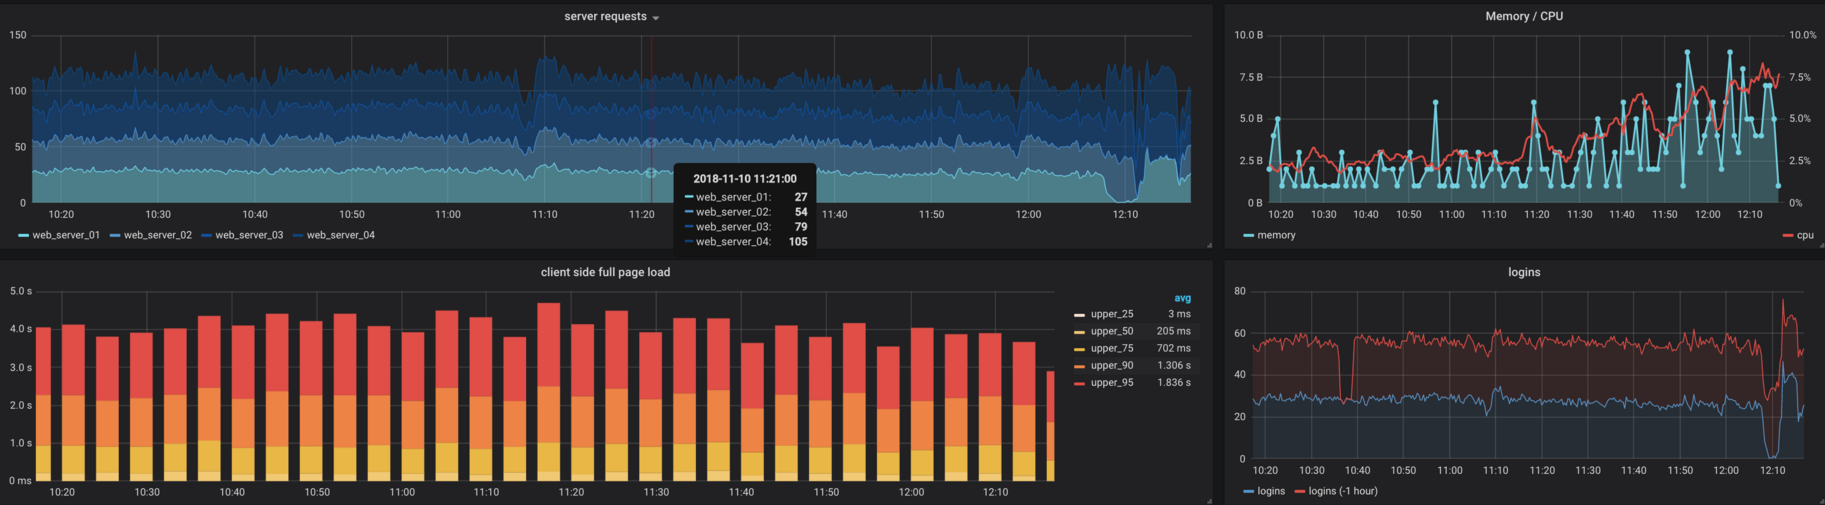
\includegraphics[width=0.97\textwidth]{grafana_panels.png}\\[0.15cm]
  {\small Requests per server, page-load latency percentiles, memory and CPU.\\
  Every panel can stay normal while every prediction is wrong.}
  \mlsyscredit{Grafana sample dashboard (``Grafana Play Home''), screenshot by Joel Kennedy, 2018, public domain, Wikimedia Commons (File:Grafana screenshot (2018).png); upper panels cropped.}
  \note{[1 min] [CORE] A real infrastructure dashboard, the sample that ships with Grafana's public demo: requests per web server, client page-load time at the 25th to 95th percentiles, memory and CPU, logins. This is the top layer of the iceberg, and it is what an on-call engineer watches. ENGAGE: which panel would have moved when Unity's model trained on a customer's bad data? None. Every server answered, fast, with normal memory. The panels describe the service, not whether its answers are right. WARN: students assume a green dashboard means a healthy model. It means a healthy service; the next three layers exist because this one cannot see the model.}
\end{frame}

\begin{frame}{Google's input checks fired on one pipeline in ten within a month}
  \centering
  \safeimg[width=0.82\textwidth,height=4.9cm,keepaspectratio]{breck_bars.pdf}\\[0.05cm]
  {\small Removing one skew found this way raised Google Play installs 2\%.}
  \mlsyscredit{Breck, Polyzotis, Roy, Whang, and Zinkevich, ``Data Validation for Machine Learning,'' SysML 2019, Table 1 and \S6.2.}
  \note{[1.5 min] [OPTIONAL] Real measurements of the input layer. Google's data validator checks every batch against a schema, a declared list of features with their types and allowed values, in more than 700 production pipelines. Over the most recent 30 days, the bars show the share of pipelines on which each kind of anomaly fired on at least one day: a new feature column in 10 percent, out-of-domain categorical values and a missing column in 6 percent each. The right column is the share of those that were fixed, which the paper defines as two days with no anomaly of that type afterward. Google Play case: features always present in training were always missing in the serving logs; removing the skew raised app installs on the store's main landing page by 2 percent in an online experiment. ENGAGE: why are some anomalies never fixed? The paper's answer: sometimes the bad batch is allowed to age out of the window, and sometimes the on-call engineer ``might miss or ignore the alert depending on their cognitive load.'' Hold that thought for segment 3. FLEX: cutting it loses Google's measured firing rate.}
\end{frame}

\begin{frame}{A data validator names the feature and the broken expectation}
  \raggedright
  \vspace{-0.15cm}{\small\textbf{\textcolor{mlsysaccent}{Out-of-domain value}} (fired in 6\% of Google's pipelines): new data checked against the schema}\\[0.08cm]
  \hspace{0.4cm}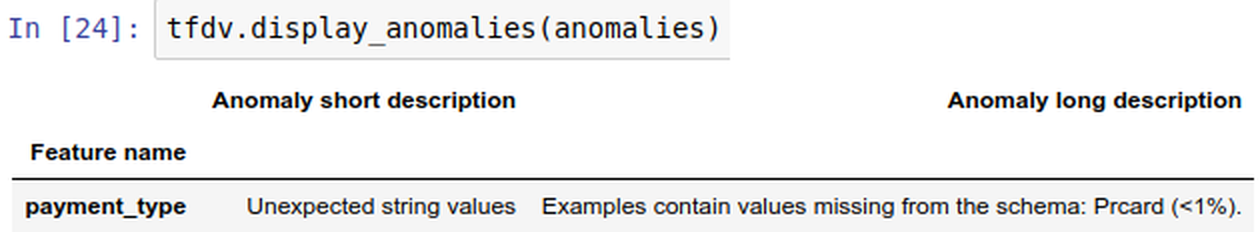
\includegraphics[width=0.74\textwidth]{tfdv_anomaly.png}\\[0.22cm]
  {\small\textbf{\textcolor{mlsysaccent}{Missing column}} (6\%): serving data checked against the same schema}\\[0.08cm]
  \hspace{0.4cm}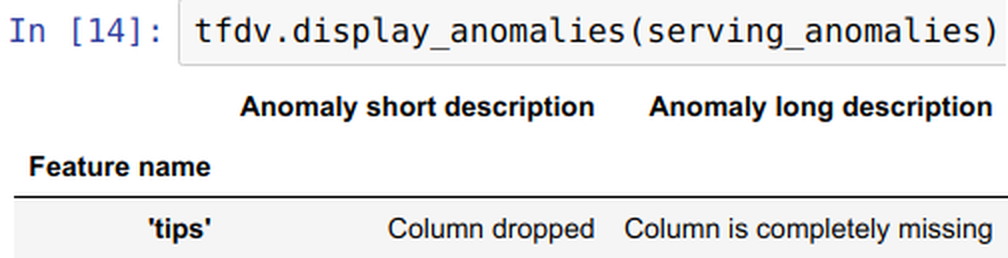
\includegraphics[width=0.592\textwidth]{tfdv_serving_anomaly.png}
  \mlsyscredit{TensorFlow Data Validation, ``Get started'' (docs/get\_started.md and docs/images/anomaly.png, serving\_anomaly.png), github.com/tensorflow/data-validation @ aaa0ae1, Apache 2.0. Rates: Breck et al.\ 2019, Table 1.}
  \note{[1.5 min] [OPTIONAL] The tool behind the bars: TensorFlow Data Validation, the open-source descendant of the validator Breck et al. measured. These are the outputs printed in its own getting-started guide. Top: new data has a payment type, Prcard, that the schema never listed, in under 1 percent of values. That is the out-of-domain categorical value that fired on 6 percent of Google's pipelines. The guide gives both exits: if the value was expected, add it to the schema; if it is a data error, fix the data before training. Bottom: the serving data has no tips column, a missing column. Here tips is the training label, absent at serving by design, so the fix is a schema environment that says so. Every alert ends in one of two decisions: repair the data or change the schema. ENGAGE: Unity's large customer sent bad data. Which row would its batch have produced? Out-of-domain or out-of-range values on the features it corrupted, at ingest, with no labels. WARN: a schema check catches values that break a declared rule; it cannot see a plausible but wrong value. That is what the drift layer is for. FLEX: cutting it loses the validator output.}
\end{frame}

\begin{frame}{A missing label is pending, not negative}
  \centering
  \mlsyssteps[width=0.92\textwidth,height=5.6cm,keepaspectratio]{join_step}{3}
  \mlsyscredit{ML Operations, \S14.5.2, joining predictions to outcomes.}
  \note{[2.5 min] [CORE] Outcome monitoring needs two logs. Step 1: the prediction log records each request's identifier, time, score, and the version that served it. The outcome log records the same identifier, the event, and when it was observed. Join them on the request identifier, and keep the served version, so each outcome is credited to the model that made the prediction, not to whichever model is live when the label arrives. Step 2: a conversion model with a fixed outcome window. A purchase inside the window is a positive. A window that closed with no purchase is a negative. A recent request whose window is still open is pending: the absence of a purchase is unknown, not a no. Step 3: so every metric and every slice reports label coverage, the share of eligible predictions whose outcomes have resolved. WARN: the common mistake is to count pending requests as negatives, which makes any new model look worse. ENGAGE: a request served this morning, with a seven-day window. Positive, negative, or pending? Pending until next week.}
\end{frame}

\begin{frame}{Check: the candidate converts 3 points worse. Roll back?}
  \mlsysactivity{Vote}{2 min}
  \begin{columns}[c]
    \begin{column}{0.46\textwidth}
      \centering\mlsyssteps[width=\textwidth,height=5.0cm,keepaspectratio]{pending_step}{2}
    \end{column}
    \begin{column}{0.50\textwidth}
      \fcolorbox{midgray}{white}{\begin{minipage}{0.94\linewidth}\raggedright
        {\scriptsize\textcolor{midgray}{Google Ads Help, ``About conversion windows''}}\\[0.04cm]
        \footnotesize ``A conversion window is the period of time after an ad interaction \ldots{} during which a conversion, such as a purchase, is recorded'' \ldots{} ``the default 30-day conversion window.''
      \end{minipage}}\\[0.2cm]
      \normalsize
      \choice{A}{Roll back the candidate}\\[0.12cm]
      \choice{B}{Retrain on recent data}\\[0.12cm]
      \answerat{2}{C}{Neither yet}\\[0.15cm]
      \uncover<2->{\small Compare cohorts whose outcome windows have closed, and report coverage.}
    \end{column}
  \end{columns}
  \mlsyscredit{Rule: ML Operations, \S14.5.2. Values illustrative. Quote: support.google.com/google-ads/answer/3123169, retrieved 19 Oct 2026.}
  \note{[2 min] [OPTIONAL] Outcome windows are a setting in real systems: Google Ads records a purchase only inside the conversion window, 30 days by default. Suppose the same window here. The candidate has served for 2 days; the incumbent's numbers cover the previous 30. Measured conversion is 10 percent for the incumbent and 7 percent for the candidate. These values are illustrative; the rule is the chapter's. ENGAGE: vote, one minute with a neighbor, vote again. Step 2: C. Most of the candidate's requests are still pending, so its conversion is counted mostly from closed windows that happen to be early, and the missing purchases inside open windows are unknown. Compare cohorts with matured windows under the same horizon, and report label coverage beside every number. The chapter: an apparent drop caused by comparing pending outcomes with completed ones does not justify retraining; it calls for completing the window. WARN: students who pick A treat a lower number as evidence. It is evidence only at equal coverage. FLEX: cutting it loses the rollback vote.}
\end{frame}

\begin{frame}{Per-feature monitors miss a reversed relationship}
  \centering
  \mlsyssteps[width=0.88\textwidth,height=5.5cm,keepaspectratio]{joint_step}{3}
  \mlsyscredit{ML Operations, \S14.5.2 (feature distribution monitoring).}
  \note{[2 min] [OPTIONAL] The chapter's counterexample. Step 1: two binary sensor flags. Each is on half the time in training and half the time in serving, so a monitor that checks each feature's histogram reports no change. Step 2: in training, the flags agree: half the population has both off, half has both on. Step 3: in serving, they disagree: half has A on and B off, half the reverse. The relationship has reversed while each flag's own histogram stayed the same. ENGAGE: would Part 1's parity replay catch this? No. Training and serving compute every feature the same way; the population changed. The fix is to monitor selected feature pairs, cohorts, or a joint statistic; labels are still needed to say whether the change hurts. One more input-layer control the chapter shows: a freshness rule that falls back to a default when a feature is more than 6 hours old (listing 4). LINK: Lecture 4b computed K-S and PSI on one feature; this slide shows what one feature cannot see. Land the segment: each layer sees a different failure at a different delay, and a missing label is pending, not wrong.}
\end{frame}

% =============================================================================
% SECTION: HOW FAST
% =============================================================================
\mlsysnote{[0.5 min] [CORE] Outcomes are the only layer that confirms accuracy fell. How long do they take?}
\mlsysdivider{How long before we can confirm the model got worse?}{ML Operations, \S14.5.2, Napkin Math 14.2 and 14.3}
\section{How Fast}

\begin{frame}{Half the drop needs about four times the evidence}
  \centering
  \mlsyssteps[width=0.78\textwidth,height=5.2cm,keepaspectratio]{evidence_step}{2}\\[0.05cm]
  {\small 95\% confidence, 80\% power, from 95\% accuracy (derived).}
  \mlsyscredit{Counts derived with the binomial sizing of Lecture 12b. Budget: ML Operations, Napkin Math 14.2.}
  \note{[2.5 min] [CORE] How many labeled outcomes does it take to confirm that a 95 percent model got worse? Step 1: derived with the same sizing Lecture 12b used for test sets, at 95 percent confidence and 80 percent power (an 80 percent chance of catching a real drop of that size). A 5-point drop needs about 185 outcomes; 2 points, about 1,030; 1 point, about 3,930. The evidence needed grows as one over the drop squared, because sampling noise shrinks only as one over the square root of the count: halve the drop and you need about four times the outcomes. Step 2: the chapter's policy budgets 1,000 outcomes to confirm a 5-point drop, above the statistical floor, to allow for noisy labels, outcomes that are not independent, and checks on every slice. ENGAGE: a team wants to catch a 0.5-point drop. How many outcomes? About 15,300 (derived); four times 3,930, about 15,700, is the quick estimate. LINK: Lecture 12b owns the formula; do not derive it again. WARN: students read the budget as a statistical law. It is a policy above the floor.}
\end{frame}

\begin{frame}[t]{Estimate: how long until a drop is confirmed?}
  \mlsysactivity{Estimate}{2 min}
  \centering
  \only<1|handout:0>{\vspace{0.6cm}\begin{mlsyscard}{mlsysaccent}\normalsize
    \textbf{Given:} 1,000 labeled outcomes confirm a 5-point drop.\\[0.1cm]
    How long at 1 label per second? At 100 per day? For a fraud model?
  \end{mlsyscard}}%
  \only<2-|handout:1>{{\small Time to confirm = label delay + outcomes needed / label rate (derived)}\\[0.1cm]
  \only<2|handout:0>{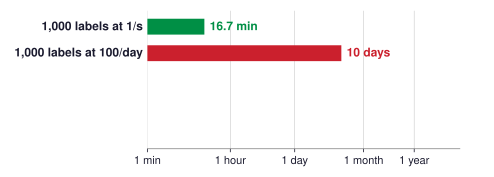
\includegraphics[width=0.95\textwidth,height=4.6cm,keepaspectratio]{delay_step1}}%
  \only<3-|handout:1>{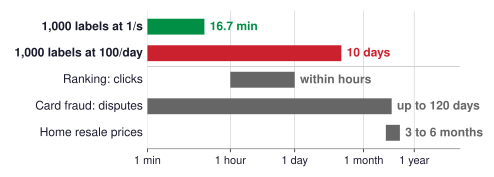
\includegraphics[width=0.95\textwidth,height=4.6cm,keepaspectratio]{delay_step2}}}
  \mlsyscredit{ML Operations, Napkin Math 14.2, \S14.1. Visa Core Rules, 18 April 2026, table 11-29. Zillow Group Q3 2021 shareholder letter.}
  \note{[3.5 min] [CORE] ENGAGE: one minute by hand. Step 2: at 1 label per second, 1,000 seconds, about 16.7 minutes; at 100 labels a day, 10 days (Napkin Math 14.2). Same test, same tooling, a factor of 864 apart. Step 3: and the clock does not start until labels exist. Clicks arrive within hours. For card-absent fraud, Visa's rules let the card issuer open a dispute up to 120 calendar days after the transaction is processed, so a fraud label can arrive four months late. Zillow's resale prices arrived three to six months after each purchase (Part 1). The sum on the slide is our derivation from the chapter's two statements: evidence arrives at the label rate, and labels lag traffic. ENGAGE: the ranking service, the low-traffic model, the fraud model: how long each? About 17 minutes plus a few hours; 10 days; up to about four months plus the collection time. WARN: students who answer ``one day, because we check daily'' confuse the check's cadence with the evidence's arrival. No tool removes a label delay; only a label-free signal or an input check can move earlier.}
\end{frame}

\begin{frame}{Label-free tests see a large shift in 20 samples}
  \centering
  \mlsyssteps[width=0.88\textwidth,height=5.5cm,keepaspectratio]{rabanser_step}{2}
  \mlsyscredit{Rabanser, G\"unnemann, and Lipton, ``Failing Loudly,'' NeurIPS 2019, Table 2a: label-free detection (univariate tests on softmax outputs), MNIST and CIFAR-10, simulated shifts. Time rows derived.}
  \note{[2.5 min] [OPTIONAL] The way to move earlier than the labels: test whether the inputs or the model's outputs changed. Rabanser et al. simulated shifts of three sizes on image datasets and asked how often a statistical test detects them from a given number of new samples. Their best detector needs no labels: it tests whether the model's own output scores changed. Read the axes: samples on a log scale, with the time to collect them at 1 per second and at 100 per day. Step 1: large shifts pass 50 percent detection at 20 samples; medium ones need about 500. Step 2: small shifts reach only 40 percent at 1,000 samples and 54 percent at 10,000. ENGAGE: at 100 samples a day, how long to beat a coin flip on a small shift? About 100 days. WARN: a label-free test says the inputs moved, not that accuracy fell. It runs at traffic speed, not label speed, which is why it is the early warning and outcomes are the confirmation.}
\end{frame}

\begin{frame}[t]{Estimate: a month of silent failure costs 28 times a day}
  \mlsysactivity{Estimate}{2 min}
  \centering
  \begin{mlsyscard}{mlsysaccent}\small
    \textbf{Given:} a recommender earns \$50M a year. A skew bug cuts conversions 5\%.\\
    It is found at a monthly review (28 days), or by a daily check (1 day).
  \end{mlsyscard}
  \vspace{0.1cm}
  \uncover<2->{\safeimg[width=0.85\textwidth,height=2.4cm,keepaspectratio]{silent_cost.pdf}\\[0.05cm]
  {\small \$184,932 more per incident; about \$739,726 a year at 4 incidents.}}
  \mlsyscredit{ML Operations, Napkin Math 14.3.}
  \note{[2 min] [OPTIONAL] What each day of delay costs. ENGAGE: estimate the loss for each case. Step 2: \$50 million times 0.05 times 28 over 365 is \$191,781; with a daily check, \$6,849. The difference is \$184,932 per incident, about \$739,726 a year at four incidents. WARN: the common error is to forget the 28/365 and answer \$2.5 million, a whole year's loss. Then the chapter's caveat: the calculation assumes the incident starts just after a check and is repaired the moment it is found; label delay, diagnosis, and recovery come on top. Combine with the last slide: a daily check on a model whose labels arrive in 120 days does not detect in one day. The saving belongs to the label-free and input-layer monitors. Land the segment: confirmation time is the label delay plus the evidence a drop needs divided by the rate labels arrive; halving the drop quadruples the evidence, and every day of waiting has a price.}
\end{frame}

% =============================================================================
% SECTION: WHEN TO ALERT
% =============================================================================
\mlsysnote{[0.5 min] [CORE] Fast detection is useless if it pages on every harmless change. When should a monitor wake someone?}
\mlsysdivider{When should a monitor wake someone up?}{ML Operations, \S14.5.2 and \S14.7.1}
\section{When to Alert}

\begin{frame}{At a million samples, almost any shift is significant}
  \centering
  \mlsyssteps[width=0.78\textwidth,height=5.3cm,keepaspectratio]{ks_step}{2}
  \mlsyscredit{Critical value $1.36\sqrt{2/n}$, 95\% (Lecture 4b, Napkin Math 4.5); the value at 1,000,000 derived. Gate: ML Operations, listing 2.}
  \note{[2.5 min] [OPTIONAL] Lecture 4b used the Kolmogorov-Smirnov (K-S) test, which compares two distributions by their largest gap, to flag a drifted feature. Step 1: the gap the test needs before it calls a difference significant falls as one over the square root of the sample size: 0.061 for 1,000 samples on each side, 0.006 for 100,000 (both from Lecture 4b), and 0.0019 for 1,000,000 (derived). Step 2: the chapter's release policy pauses promotion only when the statistic exceeds 0.1. A monitor comparing a day of serving traffic with the training set rejects equality for shifts 52 times smaller than that gate (derived). ENGAGE: is a 0.002 shift in a feature's distribution one you would retrain for? No. The detection is real; paging on it is the error. WARN: students hear ``significant'' as ``important.'' At production scale significance is free, so an alert needs an effect size. LINK: Lecture 4b owns the test itself; this slide adds only the scale argument.}
\end{frame}

\begin{frame}{A monitor with nothing to find still pages every day}
  \begin{columns}[c]
    \begin{column}{0.55\textwidth}
      \centering
      \safeimg[width=\textwidth,height=3.4cm,keepaspectratio]{falsealarm.pdf}\\[0.15cm]
      \uncover<2->{{\small\textbf{Measured:} ICU monitor alarms,\\461 patients, 31 days}\\[0.05cm]
      \safeimg[width=\textwidth,height=1.0cm,keepaspectratio]{icu.pdf}}
    \end{column}
    \begin{column}{0.43\textwidth}
      \centering
      \uncover<2->{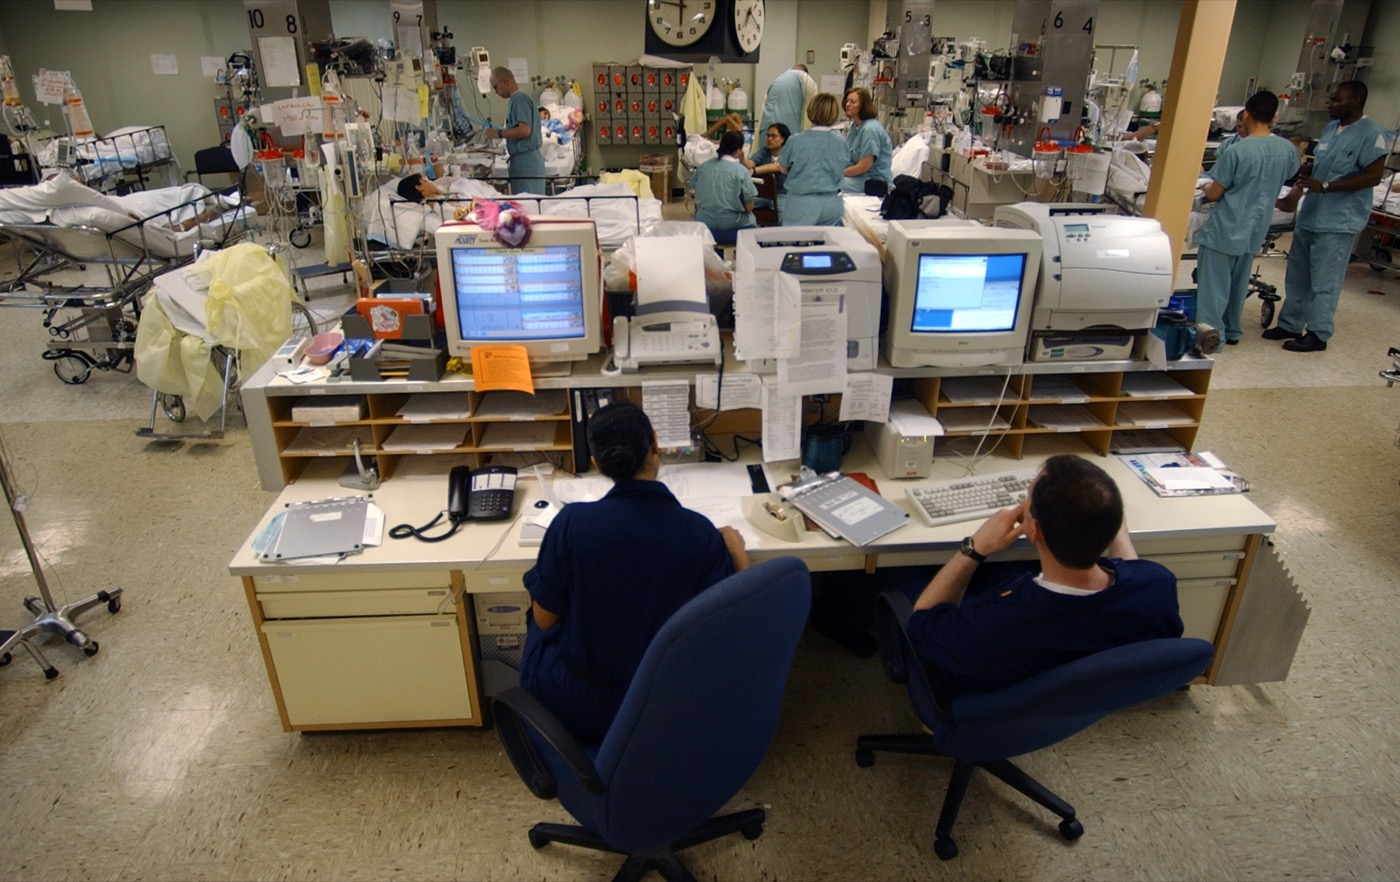
\includegraphics[width=\textwidth]{icu_central_station.jpg}\\[0.05cm]
      {\footnotesize A central ICU station: every bed's heart monitor on one desk (USNS Comfort, 2003)}}
    \end{column}
  \end{columns}
  \mlsyscredit{False alerts derived from Napkin Math 14.5's 150 series. Drew et al., PLOS ONE 2014. Photo: U.S. Navy, PH1 Shane T. McCoy, 2003, public domain, Wikimedia Commons.}
  \note{[2.5 min] [CORE] Step 1: the chapter's monitoring budget watches one model in three deployment variants with 50 metrics each, 150 series (Napkin Math 14.5). Suppose nothing has changed and each series is tested once a day. At a per-test false-positive rate of 0.05, the monitor raises 7.5 false alerts a day; at 0.01, 1.5; at 0.001, 0.15, about one a week (derived: 150 times the rate; 1.05 a week). ENGAGE: what does a lower rate give up? It misses smaller real changes. Step 2: what an untuned threshold does to people, measured. Drew et al. recorded 2,558,760 unique alarms from 461 adult intensive-care patients in 31 days; of 12,671 annotated arrhythmia alarms, 88.8 percent were false. The paper calls the result alarm fatigue: staff stop responding. The photo shows the workplace: a central station where two people watch every bed's heart monitor (a Navy hospital ship's ICU, not the hospital Drew et al. studied). WARN: a threshold is a budget of false alarms, set together with an effect size and an owner, not a constant copied from a textbook. The chapter's remedies for alert fatigue: consolidate related alerts, use thresholds that follow weekly and seasonal patterns, retire alerts that are rarely actionable, and require a follow-up ticket before any alert is silenced (\S14.7.1). FLEX: step 2 is cuttable.}
\end{frame}

\begin{frame}[fragile]{A real alert rule: a threshold, a hold time, and a severity}
  \begin{mlsyscard}{mlsysaccent}
\begin{semiverbatim}\footnotesize
  - alert: HighRequestLatency
    expr: job:request_latency_seconds:mean5m\{job="myjob"\} \alert<2->{> 0.5}
    \alert<3->{for: 10m}
    keep_firing_for: 5m
    labels:
      \alert<4->{severity: page}
\end{semiverbatim}
  \end{mlsyscard}
  \vspace{0.15cm}
  \small
  \uncover<2->{\textbf{\textcolor{mlsysaccent}{expr}}: the effect size that matters, mean latency over 5 minutes above 0.5 s}\\[0.15cm]
  \uncover<3->{\textbf{\textcolor{mlsysaccent}{for}}: the alert stays pending until the condition has held 10 minutes; shorter blips never page}\\[0.15cm]
  \uncover<4->{\textbf{\textcolor{mlsysaccent}{severity}}: a label that routing turns into a page for the on-call, or a ticket}
  \mlsyscredit{Prometheus docs, ``Alerting rules'' (docs/configuration/alerting\_rules.md), github.com/prometheus/prometheus @ v3.15.0, Apache 2.0; one rule quoted exactly, group header and annotations omitted.}
  \note{[1.5 min] [OPTIONAL] The example rule from the Prometheus documentation, the alerting system most infrastructure teams run. Step 2: expr is the threshold, written as an effect size: mean request latency over five minutes above 0.5 seconds. Step 3: the for clause. The documentation: Prometheus waits until the alert ``continues to be active during each evaluation for 10 minutes before firing''; until then the alert is pending. That clause is the trade from the last slide in one line: every minute of hold time adds a minute of detection delay and removes every false alarm shorter than it. keep\_firing\_for holds the alert 5 minutes after it clears, so it does not flap. Step 4: severity: page is a label; a routing rule decides that a page wakes the on-call engineer and a lower severity becomes a ticket. ENGAGE: the 150 series of the last slide fire 7.5 false alerts a day at a 0.05 rate. Name two fields in this rule that cut that number. A higher threshold in expr, and a longer for. WARN: an ML drift rule has the same shape, but its expr is a drift statistic, and its for must be long enough for the samples the statistic needs. FLEX: cutting it loses the real alert rule.}
\end{frame}

\begin{frame}{Check: the age feature's PSI is 0.029. Page, ticket, or log?}
  \mlsysactivity{Vote}{2 min}
  \begin{columns}[c]
    \begin{column}{0.47\textwidth}
      \centering\safeimg[width=\textwidth,height=3.4cm,keepaspectratio]{psi_bars.pdf}\\[0.1cm]
      {\footnotesize $\text{PSI} = \sum (s_i - t_i)\ln(s_i/t_i)$\\[0.04cm]
      66+: $0.03 \times \ln 1.3 = 0.0079$; six bins: 0.029}\\[0.15cm]
      {\small\choice{A}{page}\quad\choice{B}{ticket}\quad\answerat{2}{C}{log}}
    \end{column}
    \begin{column}{0.51\textwidth}
      \centering\only<1|handout:0>{\vspace{5.6cm}}%
      \only<2|handout:0>{\safeimg[width=\textwidth,height=5.6cm,keepaspectratio]{psi_ladder_step1.pdf}}%
      \only<3-|handout:1>{\safeimg[width=\textwidth,height=5.6cm,keepaspectratio]{psi_ladder_step2.pdf}}
    \end{column}
  \end{columns}
  \mlsyscredit{ML Operations, table 13, \S14.5.2 (PSI bands; conventions, not laws), and table 19 (illustrative severity policy). $s_i$, $t_i$: serving and training shares of bin $i$ (Lecture 4b).}
  \note{[2.5 min] [CORE] The chapter's ranking service watches user age. As the audience aged, four bins moved by 3 percentage points and two by 2. The population stability index (PSI), from Lecture 4b, sums one term per bin, (serving minus training) times the log of their ratio; for the 66-and-over bin, 0.03 times ln 1.3, or 0.0079. The six terms total 0.029 (table 13). ENGAGE: page the on-call engineer, open a ticket for the owner, or log it? Vote. Step 2: C. The chapter turns the usual PSI bands into an escalation policy: below 0.1, log it and keep watching outcomes and critical slices; 0.1 to 0.25, investigate the pipeline and the population; 0.25 or more, notify the owning team. Step 3: a page needs a severity, and severity needs impact, which PSI alone does not show. The chapter's illustrative policy gives each level a deadline and an owner: 15 minutes when the service is down, 1 hour for broad harm, 4 hours when a fallback works, 24 hours with no observed impact. WARN: students who say ``page'' read a visible histogram change as harm. Land the segment: an alert needs an effect size, a false-alarm budget, an owner, and a deadline; a drift band opens an investigation, never a retraining run.}
\end{frame}

% =============================================================================
% SECTION: RETRAIN OR WAIT
% =============================================================================
\mlsysnote{[0.5 min] [CORE] The alert says the world moved. Is a retraining run worth its cost, and how often?}
\mlsysdivider{When is a retraining run worth its cost?}{ML Operations, \S14.6}
\section{Retrain or Wait}

\begin{frame}{A drift alert opens a question; the gate decides}
  \centering
  \mlsyssteps[width=0.82\textwidth,height=5.4cm,keepaspectratio]{gate_step}{3}
  \mlsyscredit{ML Operations, listing 5, equation 10, and \S14.6.1.}
  \note{[2.5 min] [CORE] Step 1: the chapter's retraining gate (listing 5) as a balance. On the left, the value a run would recover, estimated from the measured quality loss, feature drift, and the shift in predictions. On the right, the cost of a run: compute, validation, deployment, and the expected cost of a bad rollout (equation 10). A drift alert adds evidence to the left pan; it does not decide. Step 2: the gate runs a training job only when value exceeds cost and fresh validation data exist to test the result. Step 3: three policies for when the gate is asked. Scheduled runs on a calendar: simple, but it spends runs in quiet weeks and reacts slowly between them. Triggered runs on evidence: it saves runs but depends on fast labels or good proxies. Continuous updates the weights as labels arrive: least staleness, but corrupted or adversarial data can reach the weights before anyone looks. ENGAGE: which policy would have trained on Unity's bad customer batch fastest? Continuous. WARN: automated runs with automated promotion is one of the chapter's fallacies.}
\end{frame}

\begin{frame}{Production teams retrain from hourly to every few months}
  \begin{columns}[c]
    \begin{column}{0.38\textwidth}
      \centering\safeimg[width=\textwidth,height=5.2cm,keepaspectratio]{fb_cadence.pdf}
    \end{column}
    \begin{column}{0.58\textwidth}
      \centering\uncover<2->{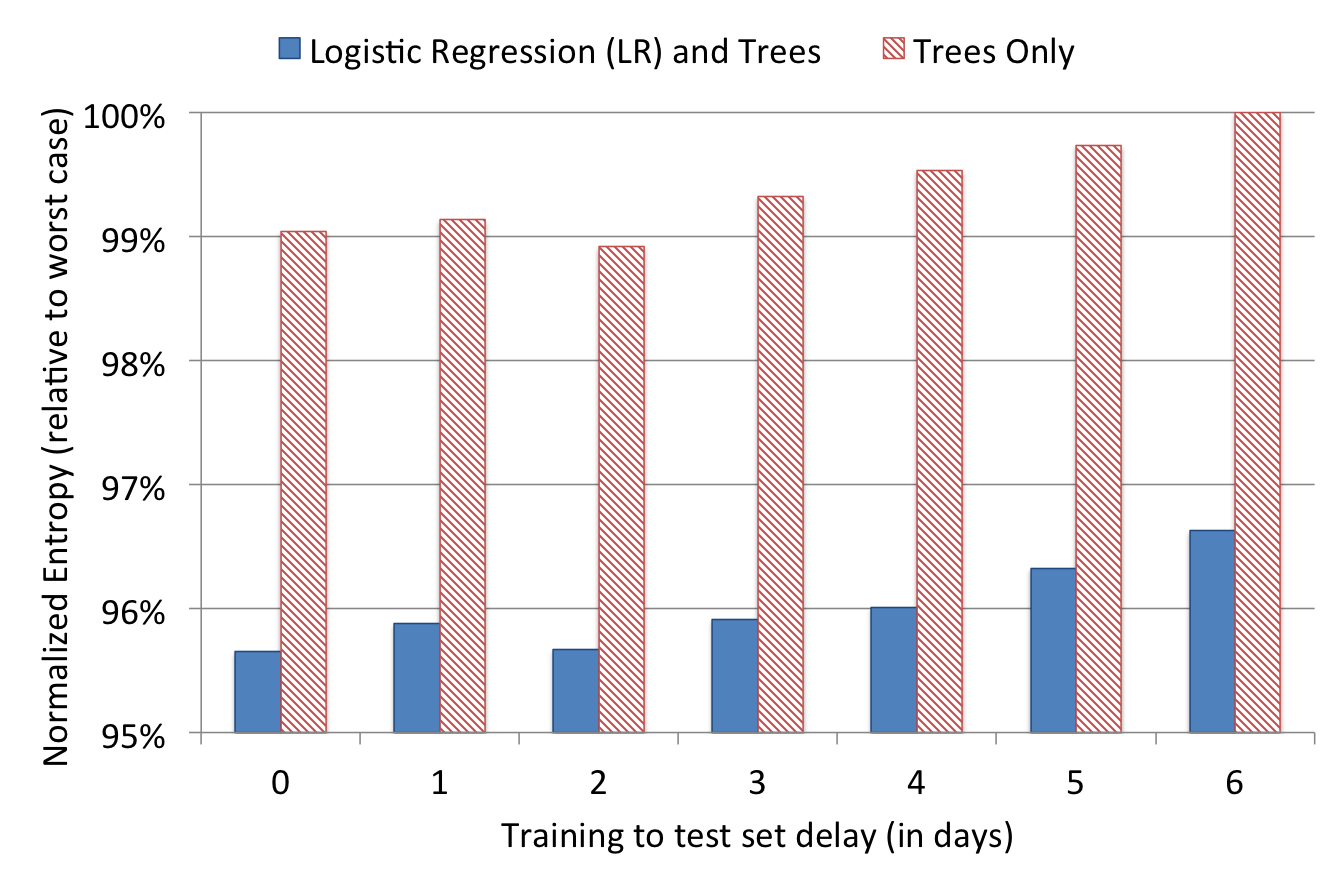
\includegraphics[width=\textwidth,height=5.3cm,keepaspectratio]{he_fig2.png}\\[0.05cm]
      {\footnotesize He et al., Figure 2: lower is better}}
    \end{column}
  \end{columns}
  \mlsyscredit{Left: Hazelwood et al., HPCA 2018, Table II. Right: He et al., ``Practical Lessons from Predicting Clicks on Ads at Facebook,'' ADKDD 2014, Figure 2 (the paper's image).}
  \note{[2 min] [OPTIONAL] The measured range of answers. Step 1: Facebook's 2018 report of how often its production models were retrained. Search hourly; Sigma (classifiers for site integrity and spam) several times a day; News Feed daily; translation and speech weekly; Lumos (image understanding) every few months. Same company, same hardware; cadence follows how fast each problem's world changes and what a run costs. Step 2: why the ads team trained daily. He et al. trained a click model on one day and tested it on each of the next six. This is the paper's own figure. Normalized entropy (NE) is their prediction loss, shown relative to the worst case, lower is better; the blue bars are their production design, logistic regression on tree features, and the hatched bars trees alone. Both rise as the test day moves away. The paper: training daily instead of weekly reduced NE by about 1 percent, more than most feature-engineering experiments gained. WARN: the differences look small because NE is relative; the paper's point is that 1 percent was more than most feature work gained. ENGAGE: is daily always right? The next slide derives the answer.}
\end{frame}

\begin{frame}{Each cycle without retraining loses a triangle of value}
  \centering
  \mlsyssteps[width=0.78\textwidth,height=4.5cm,keepaspectratio]{saw_step}{3}\\[0.05cm]
  \uncover<4->{\small Cost per day $= \dfrac{C}{T} + \dfrac{1}{2}\,QVA_0\gamma\, T$\quad lowest where \textbf{triangle = C}}
  \mlsyscredit{ML Operations, equations 8 to 12 and table 17 (illustrative ranking service: $QVA_0\gamma$ = \$1,128 per day per day).}
  \note{[3 min] [CORE] Step 1: accuracy decays as $A_0 e^{-\gamma t}$ (equation 8). Each day, the ranking service loses value in proportion to how far accuracy has fallen: queries per day Q, value per query of a unit of accuracy V, starting accuracy $A_0$, and decay rate $\gamma$. While the loss is small, value lost per day grows in a straight line, \$1,128 for every day since the last run, and resets when a run restores accuracy. Step 2: the loss over one cycle of length T is the triangle under that line: one half times 1,128 times T squared. Step 3: each reset costs one run, C = \$5,000. Step 4: per day, the run costs C over T and the staleness costs half of 1,128 times T. Retrain often and the first term dominates; rarely, the second. The sum is lowest where the two are equal, which is where one cycle's triangle equals one run's cost (derived from equations 11 and 12). ENGAGE: if the triangle is larger than C, should T shrink or grow? Shrink. WARN: the formula assumes gradual decay at a steady rate; a sudden drop is an incident, not a reason to retrain.}
\end{frame}

\mlsysnote{[1 min] [CORE] The key law of the lecture. Setting the triangle equal to C and solving for T gives the square root. The interval grows with the square root of the run cost and shrinks with the square root of traffic, value, and decay; quadruple any term and the interval changes by a factor of two (table 18). The approximation holds while the model loses only a small fraction of its accuracy between runs (equation 12).}
\mlsysfocus{The optimal retraining interval}{%
  $\displaystyle T^{*} \approx \sqrt{\frac{2\,C}{Q \cdot V \cdot A_0 \cdot \gamma}}$\\[0.6cm]
  {\small\textcolor{white!75}{$C$: cost of one run \quad $Q$: queries per day \quad $V$: value per query per unit accuracy}}\\[0.15cm]
  {\small\textcolor{white!75}{$A_0$: accuracy after retraining \quad $\gamma$: accuracy decay rate per day}}%
}

\begin{frame}{Estimate: retrain the ranking service every 3 days}
  \mlsysactivity{Estimate}{3 min}
  \begin{columns}[c]
    \begin{column}{0.42\textwidth}
      \begin{mlsyscard}{mlsysaccent}
        \small\textbf{Given} (illustrative)\\[0.05cm]
        $Q$ = 1,000,000/day; $V$ = \$0.50\\
        $A_0$ = 0.94; $\gamma$ = 0.0024/day\\
        $C$ = \$5,000 per run
      \end{mlsyscard}
      \footnotesize
      \wstep{2}{$QVA_0\gamma$ = \$1,128 per day per day}
      \wstep{2}{$T^* = \sqrt{10{,}000 / 1{,}128} \approx$ \textbf{2.98 days}}
      \wstep{3}{$C$ = \$1,250: about 1.5 days.}
      \wstep{3}{Accelerators: \$96 of the \$5,000 (1.9\%).}
    \end{column}
    \begin{column}{0.56\textwidth}
      \centering
      \only<1-2|handout:0>{\includegraphics[width=\textwidth,height=4.6cm,keepaspectratio]{tstar.pdf}}%
      \only<3-|handout:1>{\includegraphics[width=\textwidth,height=3.7cm,keepaspectratio]{tcost.pdf}\\[0.1cm]
      \mlsysphoto[height=1.5cm,keepaspectratio]{nvidia-h100-pcie-four.jpg}\hspace{0.2cm}%
      \begin{minipage}[c]{0.5\linewidth}\raggedright\footnotesize The run: 4 H100s $\times$ 6 h = 24 accelerator-hours, \$96\end{minipage}}
    \end{column}
  \end{columns}
  \mlsyscredit{ML Operations, eq.~12, Napkin Math 14.6, tables 17, 18, \S14.6.2; costs derived (the margin sketch marks 1 day). Photo: Geekerwan, CC BY 3.0, Commons.}
  \note{[3 min] [CORE] ENGAGE: two minutes with the card; also answer for a cheaper validation path that cuts C to \$1,250. Step 2: 1,000,000 times 0.50 times 0.94 times 0.0024 is \$1,128 of lost value per day, per day since the last run. Twice the run cost is 10,000; 10,000 over 1,128 is 8.87; its square root is 2.98, about 3 days. The plot shows the two cost curves crossing there. Step 3: the total cost per day at four cadences, derived from the same expression: daily \$5,564, every 3 days \$3,359, weekly \$4,662, monthly \$17,087. A quarter of the run cost halves the interval to about 1.5 days (table 18). Where the money goes: four H100s, the cards in the photo, for six hours is 24 accelerator-hours, \$96 at the registry's training rate, 1.9 percent of the run; validation, deployment, and rollout risk are the rest. So faster validation shortens the interval more than faster training. WARN: students who say ``daily, like News Feed'' should see that cadence is a result of costs, not a convention.}
\end{frame}

\begin{frame}{Detection delay lowers the floor a trigger actually holds}
  \centering
  \mlsyssteps[width=0.86\textwidth,height=5.4cm,keepaspectratio]{rot_step}{3}
  \mlsyscredit{After ML Operations, figure 9, redrawn from equation 8 with $\gamma$ = 0.0024/day. Days to 0.88 and the delayed resets derived.}
  \note{[2.5 min] [OPTIONAL] The chapter's comparison of a schedule and a trigger, redrawn from its decay model with the ranking service's rate. Step 1: retraining every 90 days lets accuracy fall from 0.94 to 0.757 before each reset (derived), far below a 0.88 floor. Step 2: a trigger that fires the moment accuracy touches 0.88 retrains every 27.5 days and never dips below, matching the four-week slide from 94 to 88 percent in Part 1. The chapter warns that this curve assumes no delay. Step 3: add segment 2's delays. With a 1-day delay, the reset comes at 0.878; with the 10-day delay of a low-traffic model, at 0.859 (derived). The floor a trigger actually holds is the threshold minus the decay during detection. ENGAGE: to hold a real floor of 0.88 with a 10-day delay, where must the trigger sit? About 0.901, ten days of decay above it (derived). WARN: a sudden drop with a cause inside the system, a broken transform or a bad release, goes to incident response, not retraining. Land the segment: a run pays when recovered value beats its cost; the best interval grows with the square root of that cost; detection delay sets the floor a trigger holds. FLEX: cutting it loses the detection-delay floor.}
\end{frame}

% =============================================================================
% SECTION: RESPOND
% =============================================================================
\mlsysnote{[0.5 min] [CORE] The alert has fired and it is real. What do we check first, and what does a repair restore?}
\mlsysdivider{The alert has fired. What do we check first, and what does a fix restore?}{ML Operations, \S14.7.1 and \S14.8.1}
\section{Respond}

\begin{frame}{Diagnose: click-through fell 12 percent at 2 AM}
  \mlsysactivity{Diagnose}{2 min}
  \begin{columns}[c]
    \begin{column}{0.40\textwidth}
      \centering
      \alt<2->{\causecard{GreenLine}{Data pipeline\\broke}}{\causecard{midgray}{Data pipeline\\broke}}\hspace{0.05cm}%
      \causecard{midgray}{Model\\drift}\\[0.12cm]
      \causecard{midgray}{Seasonal\\traffic}\hspace{0.05cm}%
      \causecard{midgray}{Statistical\\noise}\\[0.2cm]
      {\footnotesize No stack trace. No crashed process. Which do you check first?}\\[0.15cm]
      \uncover<2->{\footnotesize\textbf{Order:} pipeline, skew replay, slices, time pattern, then the model.}
    \end{column}
    \begin{column}{0.56\textwidth}
      \centering
      \only<1|handout:0>{\vspace{4.3cm}}%
      \only<2|handout:0>{\mlsyskitfig[width=\textwidth,height=4.3cm,keepaspectratio]{dam_D}}%
      \only<3-|handout:1>{\safeimg[width=\textwidth,height=4.6cm,keepaspectratio]{slices.pdf}}
    \end{column}
  \end{columns}
  \mlsyscredit{ML Operations, \S14.7.1, the debugging decision tree, and table 20 (illustrative).}
  \note{[3 min] [CORE] The chapter's incident: at 2:00 a.m. the on-call engineer is paged because the ranking service's click-through rate fell 12 percent in an hour. There is no error to read. ENGAGE: pairs choose which cause to check first, and why. Step 2: the data pipeline: schema changes, missing values, a changed transform. Altered inputs reach every prediction, and the check takes minutes. On the D-A-M triangle this is the data vertex. Drift rarely moves 12 percent in one hour; seasonality and noise are checked against last week's pattern. The order is the chapter's tree: pipeline integrity, then a training-serving skew replay (Part 1's request-keyed parity test), then slices, then the time pattern, and only then the model. Step 3: slices. Overall accuracy of 91 percent hides tablets at 62 percent on 5 percent of traffic. WARN: students jump to ``retrain''; retraining on broken inputs bakes the bug into the weights. LINK: feature attribution comes last and says what the model relied on, not what caused the error; Lecture 15b prices explanations, and the methods are reading.}
\end{frame}

\begin{frame}{A repair restores the whole contract, not just the weights}
  \centering
  \mlsyssteps[width=0.88\textwidth,height=5.6cm,keepaspectratio]{repair_step}{3}
  \mlsyscredit{ML Operations, \S14.7.1 (the session-duration defect on the ranking service, illustrative).}
  \note{[2.5 min] [CORE] The same alert, traced to a cause: it coincides with a serving-transform release on one host; the weights, runtime, and offline feature definition did not change. Step 1: replay the exact logged inputs through both paths. The replay reproduces Part 1's defect: training measured session length in wall-clock time, about 45 minutes on average, serving counted only foreground-active time, about 12. Step 2: the owning engineer restores the prior serving transform and its matching feature-cache namespace, checks the result on replayed requests, then exposes it through a bounded canary. Matched values agree again. Whether user outcomes recover is known only when mature outcomes arrive, days later. Step 3: two tempting moves that are not repairs. Rolling back the weights alone leaves the changed feature computation in place. Retraining now teaches the model against the defect instead of fixing it. ENGAGE: what has the replay proved, and what has it not? It proved the feature contract was broken and is restored; it has not yet proved the revenue effect. FLEX: if short, show only step 3.}
\end{frame}

\begin{frame}{An incident ends when it becomes a check}
  \mlsysactivity{Vote}{2 min}
  \centering
  {\footnotesize\textcolor{midgray}{Example postmortem, \emph{Site Reliability Engineering}, Appendix D (incident \#465; rows 1 to 6 of 9 omitted)}}\\[0.05cm]
  \fbox{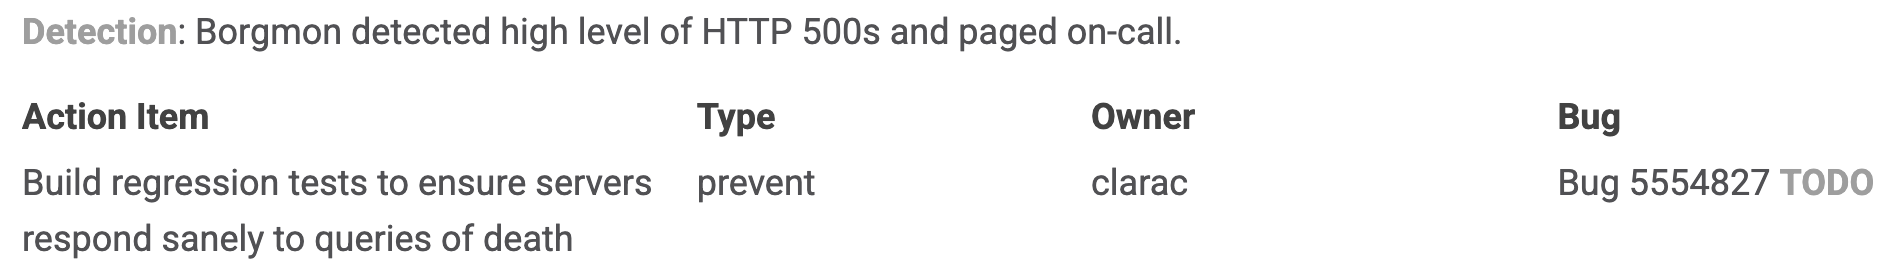
\includegraphics[width=0.9\textwidth]{sre_postmortem.png}}\\[0.15cm]
  \begin{columns}[c]
    \begin{column}{0.54\textwidth}
      \small ML Test Score audit: data 6, model 7, infrastructure 5, monitoring 1. Leadership adds two model tests. What is the score?\\[0.15cm]
      \uncover<2->{\textbf{1.} The score is the weakest category. Add schema, skew, and staleness alerts.}
    \end{column}
    \begin{column}{0.42\textwidth}
      \centering\mlsyssteps[width=\textwidth,height=2.7cm,keepaspectratio]{mlts_step}{2}
    \end{column}
  \end{columns}
  \mlsyscredit{Beyer et al., \emph{Site Reliability Engineering}, 2016, sre.google/sre-book/example-postmortem (screenshot 19 Oct 2026; CC BY-NC-ND 4.0). ML Operations, \S14.7.1, \S14.8.1; Breck et al.\ 2017.}
  \note{[3 min] [CORE] The chapter's six-phase debugging checklist (reproduce, isolate, bisect, attribute, validate, prevent) ends in Prevent: every resolved incident becomes a monitoring rule or a validation check. The SRE book's example postmortem (its Appendix D) shows what that looks like on paper; the incident, a sonnet found in a DeLorean, is plainly invented, but the fields are the book's own form. Read the Detection line: monitoring paged on HTTP 500s. Then the action item: a regression test, typed prevent, with a named owner and a bug number. That row is the incident becoming a check. The chapter's policy requires a postmortem for every P0 and P1 incident, naming the monitoring gap and the check that would have caught it earlier. ENGAGE: Google's ML Test Score has 28 tests, 7 in each of four categories, scored 0.5 for a documented manual test and 1 for an automated one. A team scores data 6, model 7, infrastructure 5, monitoring 1, and leadership proposes two more model tests. Vote on the score. Step 2: 1. The composite is the minimum category, so model tests change nothing; the next work is monitoring: alerts on schema changes, skew checks, staleness alerts. LINK: Part 1's 96 Google postmortems exist because every outage got one.}
\end{frame}

% =============================================================================
% CLOSING
% =============================================================================
\begin{frame}{Each instrument fires before the revenue report}
  \mlsysactivity{Retrieval}{3 min}
  \begin{columns}[c]
    \begin{column}{0.63\textwidth}
      \centering\safeimg[width=\textwidth,height=5.0cm,keepaspectratio]{unity_synth.pdf}
    \end{column}
    \begin{column}{0.35\textwidth}
      \footnotesize
      \only<1|handout:0>{\normalsize Close your notes. For detect, diagnose, decide, and respond, name the control from today and when it would have fired.}%
      \only<2-|handout:1>{\textbf{\textcolor{mlsysaccent}{Detect}}: schema and distribution check on each batch\\[0.08cm]
      \textbf{\textcolor{mlsysaccent}{Diagnose}}: data first; lineage names the batch\\[0.08cm]
      \textbf{\textcolor{mlsysaccent}{Decide}}: roll back to known-good data; retrain after the rebuild\\[0.08cm]
      \textbf{\textcolor{mlsysaccent}{Respond}}: the bad batch becomes a validation rule}
    \end{column}
  \end{columns}
  \mlsyscredit{Unity Software, Q1 2022 earnings call, 10 May 2022 (transcript, The Motley Fool).}
  \note{[3 min] [CORE] Back to Unity's timeline. Close your notes; two minutes in pairs. Step 2: detect: a schema and distribution check on each incoming customer batch fires at ingest, minutes after the data arrives, with no labels, while the outcome layer, revenue, reported a quarter later (segments 1 and 2). Its threshold is set on effect size and its alert has an owner and a deadline (segment 3). Diagnose: data first; lineage from Part 1 names the batch. Decide: roll back to the last model trained on known-good data, because retraining on bad data repeats the fault; retrain only after the data is rebuilt (segment 4), which is the order the CEO described. Respond: a postmortem turns the bad batch into a validation rule (segment 5). The company's own remediation sentence names the same three things: monitoring, alerting, and recovery. WARN: we do not know which of these Unity lacked; the filing does not say. The exercise asks what would have fired, not what failed.}
\end{frame}

\begin{frame}{Takeaways}
  \thumbline{thumb_layers_step4.pdf}{Each layer sees a different failure at a different delay.}\\[0.22cm]
  \thumbline{thumb_delay_step2.pdf}{Confirmation waits for the label delay, then for the evidence (1,000 outcomes: 16.7 minutes or 10 days).}\\[0.22cm]
  \thumbline{thumb_falsealarm.pdf}{An alert needs an effect size, a false-alarm budget (150 series at 0.05: 7.5 a day), and an owner.}\\[0.22cm]
  \thumbline{thumb_saw_step3.pdf}{Retrain when a cycle's lost value equals a run's cost: $T^*$ = 2.98 days here.}\\[0.22cm]
  \thumbline{thumb_repair_step3.pdf}{Check data first; restore the contract; add a check.}
  \note{[1.5 min] [CORE] One sentence per line, then ask students which slide taught each one. If short on time, read the second and the fourth.}
\end{frame}

\begin{frame}{Open questions}
  \normalsize
  \begin{itemize}\setlength{\itemsep}{0.3cm}
    \item A fraud model's labels arrive within 120 days. Should a drift alert alone ever roll it back? Who pays for an unneeded rollback?
    \item One false page a week costs an engineer's sleep; one missed failure costs \$184,932. Who should set the threshold?
    \item Continuous retraining minimizes staleness and maximizes exposure to bad data. For a model trained on customers' uploads, is any automatic retraining safe?
  \end{itemize}
  \note{[1 min] [OPTIONAL] No single answer. Take one or two responses to each, or assign one as a short written reflection. The first is about acting on label-free evidence; the second about who carries the cost of an alert policy; the third returns to Unity, whose model trained on a large customer's bad data.}
\end{frame}

\begin{frame}{Read and explore}
  \begin{columns}[c]
  \begin{column}{0.70\textwidth}
  \footnotesize
  \begin{itemize}\setlength{\itemsep}{0.04cm}
    \item \textbf{Read:} ML Operations, \S14.5, \S14.6, \S14.7.1, \S14.8.1, \S14.10; Napkin Math 14.2, 14.3, 14.5, 14.6 by hand; recompute $T^*$ for $C$ = \$1,250 and \$20,000.
    \item Breck et al., ``Data Validation for Machine Learning,'' SysML 2019.
    \item Rabanser, G\"unnemann, and Lipton, ``Failing Loudly,'' NeurIPS 2019.
    \item Beyer et al. (eds.), \emph{Site Reliability Engineering}, 2016, ch.~6 and 15.
    \item Drew et al., ``Alarm Fatigue with Physiologic Monitor Devices,'' PLOS ONE 2014.
    \item Breck et al., ``The ML Test Score,'' IEEE Big Data 2017.
    \item \textbf{Try:} the TensorFlow Data Validation ``Get started'' guide; Prometheus ``Alerting rules.''
  \end{itemize}
  \end{column}
  \begin{column}{0.28\textwidth}
    \centering\fbox{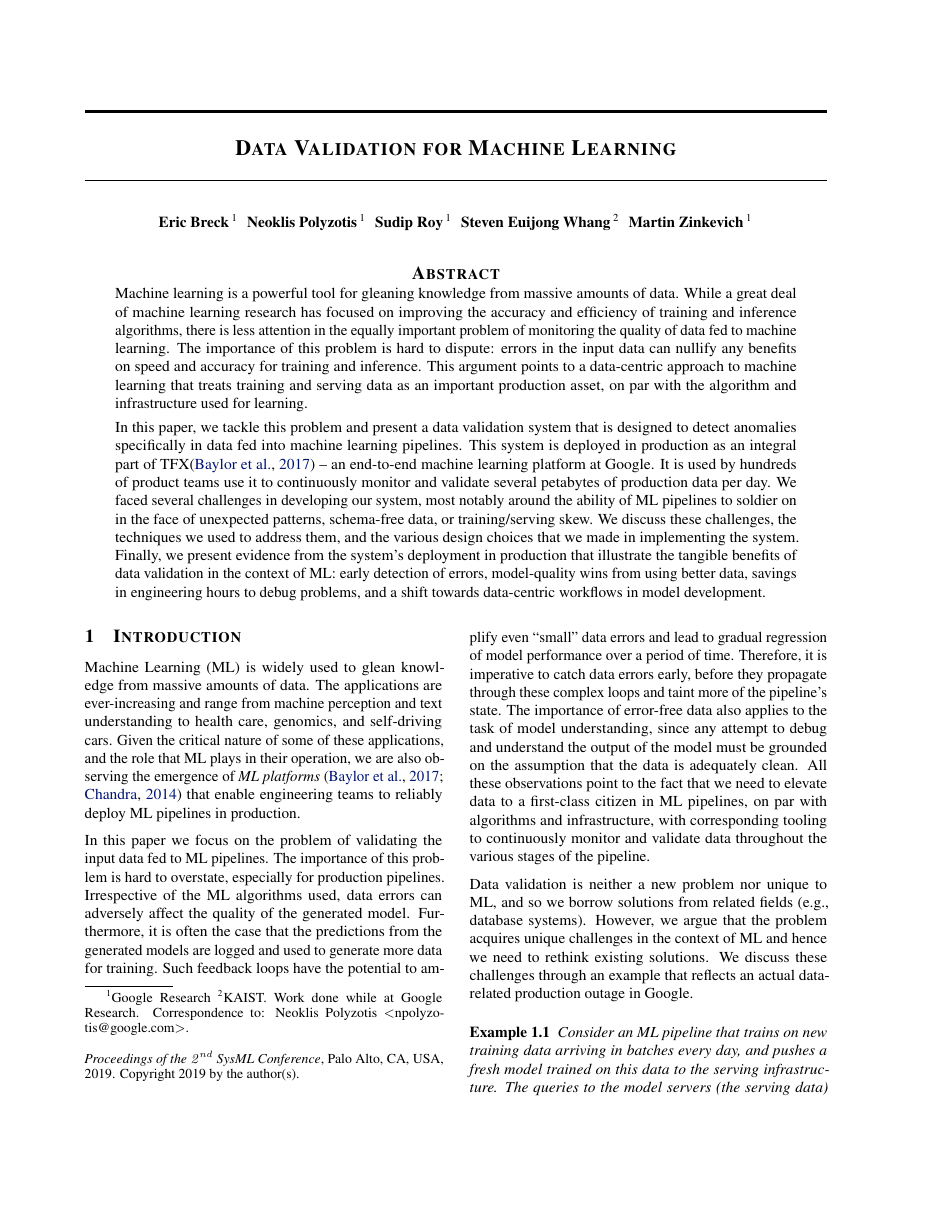
\includegraphics[height=4.3cm,keepaspectratio]{breck2019_p1.png}}\\[0.05cm]
    {\scriptsize Breck et al.\ 2019, first page}
  \end{column}
  \end{columns}
  \mlsyscredit{Breck, Polyzotis, Roy, Whang, and Zinkevich, ``Data Validation for Machine Learning,'' Proceedings of MLSys 2019 (proceedings.mlsys.org), p.~1.}
  \note{[0.5 min] [CORE] The chapter first, with Checkpoints 14.3 and 14.4 and the self-check questions for \S14.5 to \S14.8. Breck et al. 2019 shows how Google validates every batch against a schema. Rabanser et al. measures how many samples drift detection needs. The SRE book's chapter 6 says what makes an alert worth a page; chapter 15 describes blameless postmortems (free online at sre.google). Drew et al. measures alarm fatigue. The ML Test Score is the 28-test rubric. FLEX: add the lab your course uses for monitoring.}
\end{frame}

\begin{frame}[c]
  \begin{columns}[c]
    \begin{column}{0.34\textwidth}
      \centering\mlsyskitfig[width=\textwidth,height=4.2cm,keepaspectratio]{stack_operations}
    \end{column}
    \begin{column}{0.62\textwidth}
      {\small\textcolor{lightgray}{NEXT LECTURE \textbar{} RESPONSIBLE ENGINEERING, PART 1}}\\[0.5cm]
      {\Large\bfseries The system does what it was told.\\[0.1cm]Can it still cause harm?}\\[0.4cm]
      {\normalsize\textcolor{midgray}{Monitoring checks a model against its objective. Lecture 15 checks the objective.}}
    \end{column}
  \end{columns}
  \note{[0.5 min] [CORE] Close on Lecture 15's question. Two lectures kept a model faithful to its objective: rebuilt exactly, released safely, watched, and repaired. Next time asks what happens when the objective itself is wrong and the system does exactly what it was told. Fairness gates, per-group monitoring, and feedback loops that amplify bias belong there. Ask students to read Responsible Engineering before then.}
\end{frame}

\end{document}
